\begin{frame}{How to train a neural network?}
Train = optimize parameters ($w_1, w_2, \ldots, w_n, b$) for each neuron.

\manip Get a \textbf{training dataset} = examples of inputs $\vec{x}_i$ with corresponding outputs $y_i$
\manip Compare the model predictions $F(\vec{x}_i)$ to the true values $y_i$
\submanip Define a \textbf{loss function} $L$ such that its minimum is reached when $F(\vec{x}_i) = y_i$
\submanip Change the parameters a bit, aiming at minimizing $L\left( F(\vec{x}_i), y_i \right)$
\submanip Repeat
\begin{center}
When to stop training?
\end{center}

\end{frame}

\begin{frame}
\begin{center}
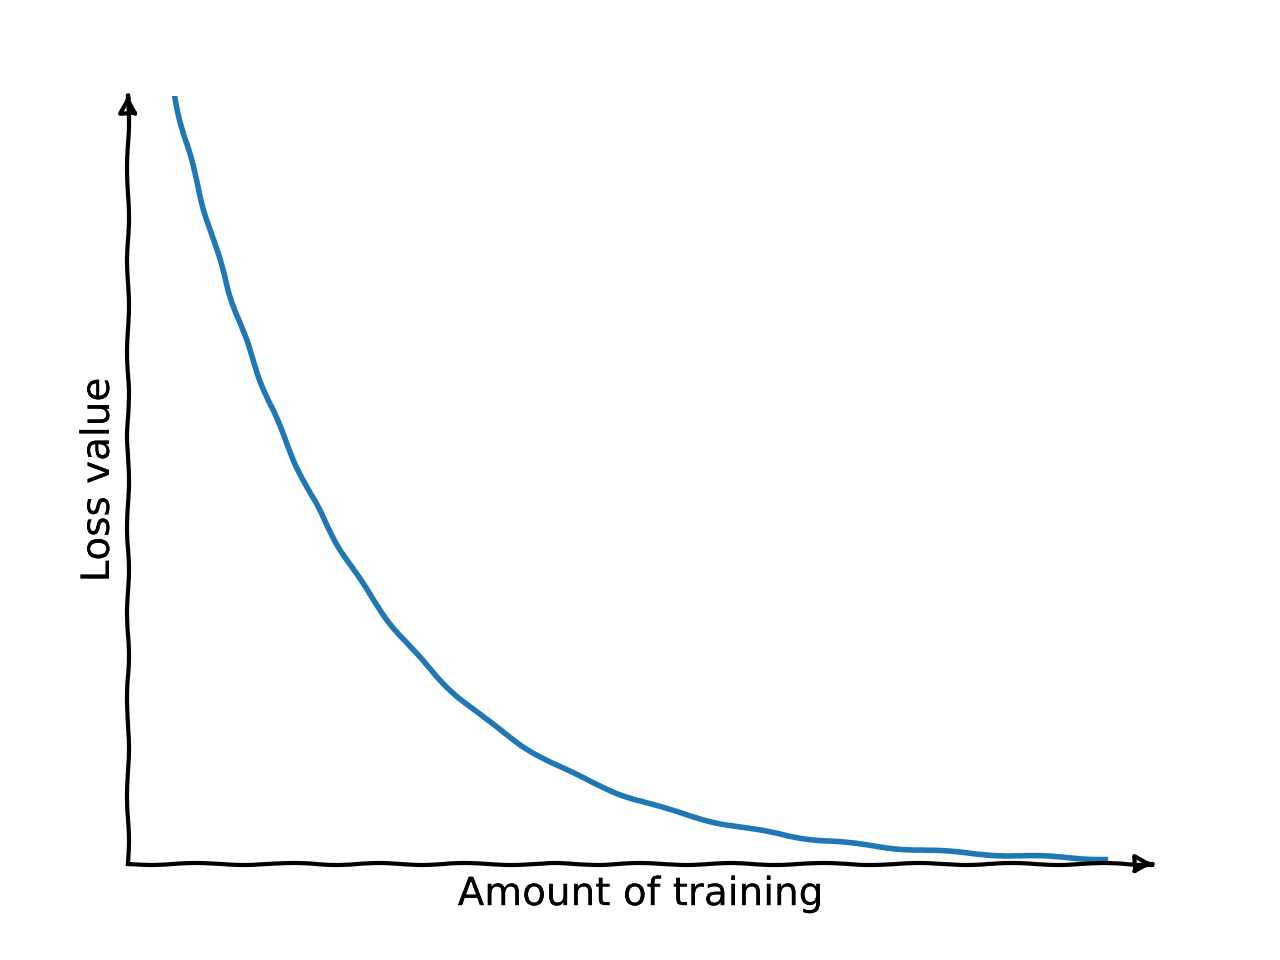
\includegraphics[width=\graphw, height=\graphh, keepaspectratio, trim = 1cm 5mm 1cm 1cm, clip]{\PhDthesisdir/plots_and_images/my_plots/ML/overfitting_and_early_stopping/overfitting_explained-1.png}
\end{center}
\end{frame}
\begin{frame}\addtocounter{framenumber}{-1}
\begin{center}
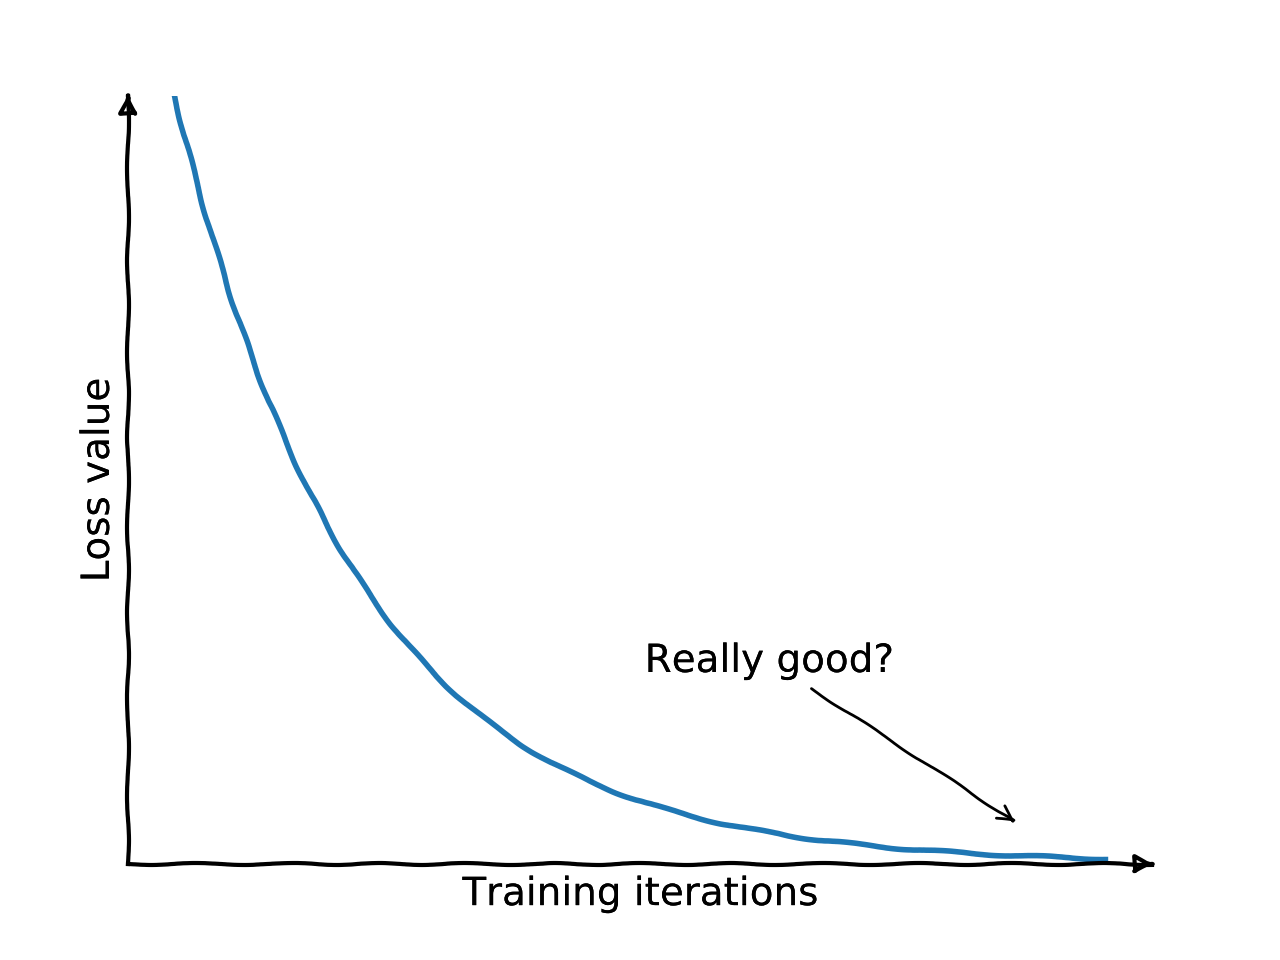
\includegraphics[width=\graphw, height=\graphh, keepaspectratio, trim = 1cm 5mm 1cm 1cm, clip]{\PhDthesisdir/plots_and_images/my_plots/ML/overfitting_and_early_stopping/overfitting_explained-2.png}
\end{center}
\end{frame}
\begin{frame}\addtocounter{framenumber}{-1}
\begin{center}
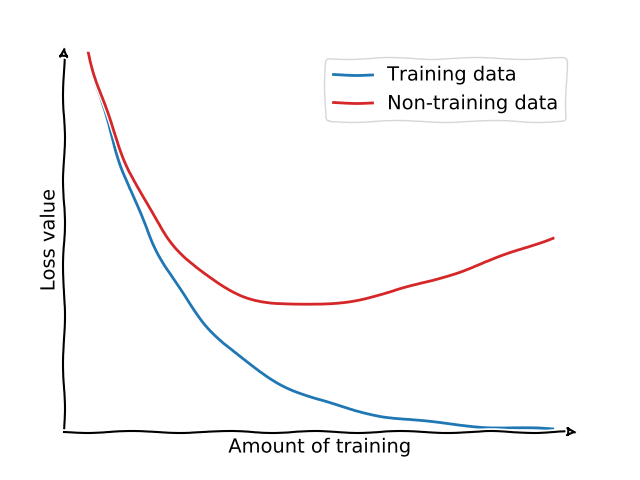
\includegraphics[width=\graphw, height=\graphh, keepaspectratio, trim = 1cm 5mm 1cm 1cm, clip]{\PhDthesisdir/plots_and_images/my_plots/ML/overfitting_and_early_stopping/overfitting_explained-3.png}
\end{center}
\end{frame}
\begin{frame}\addtocounter{framenumber}{-1}
\begin{center}
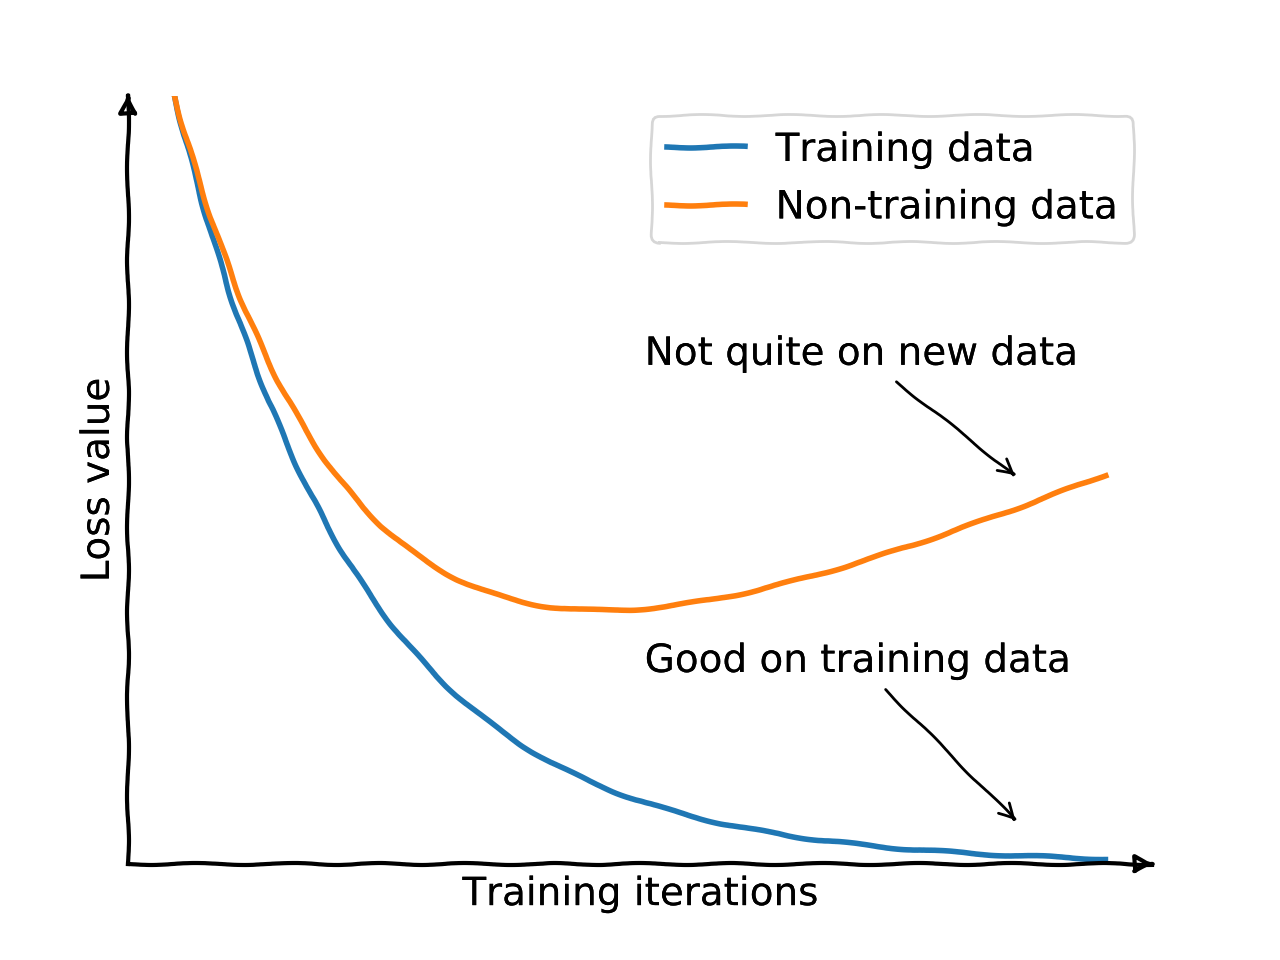
\includegraphics[width=\graphw, height=\graphh, keepaspectratio, trim = 1cm 5mm 1cm 1cm, clip]{\PhDthesisdir/plots_and_images/my_plots/ML/overfitting_and_early_stopping/overfitting_explained-4.png}
\end{center}
\end{frame}
\begin{frame}\addtocounter{framenumber}{-1}
\begin{center}
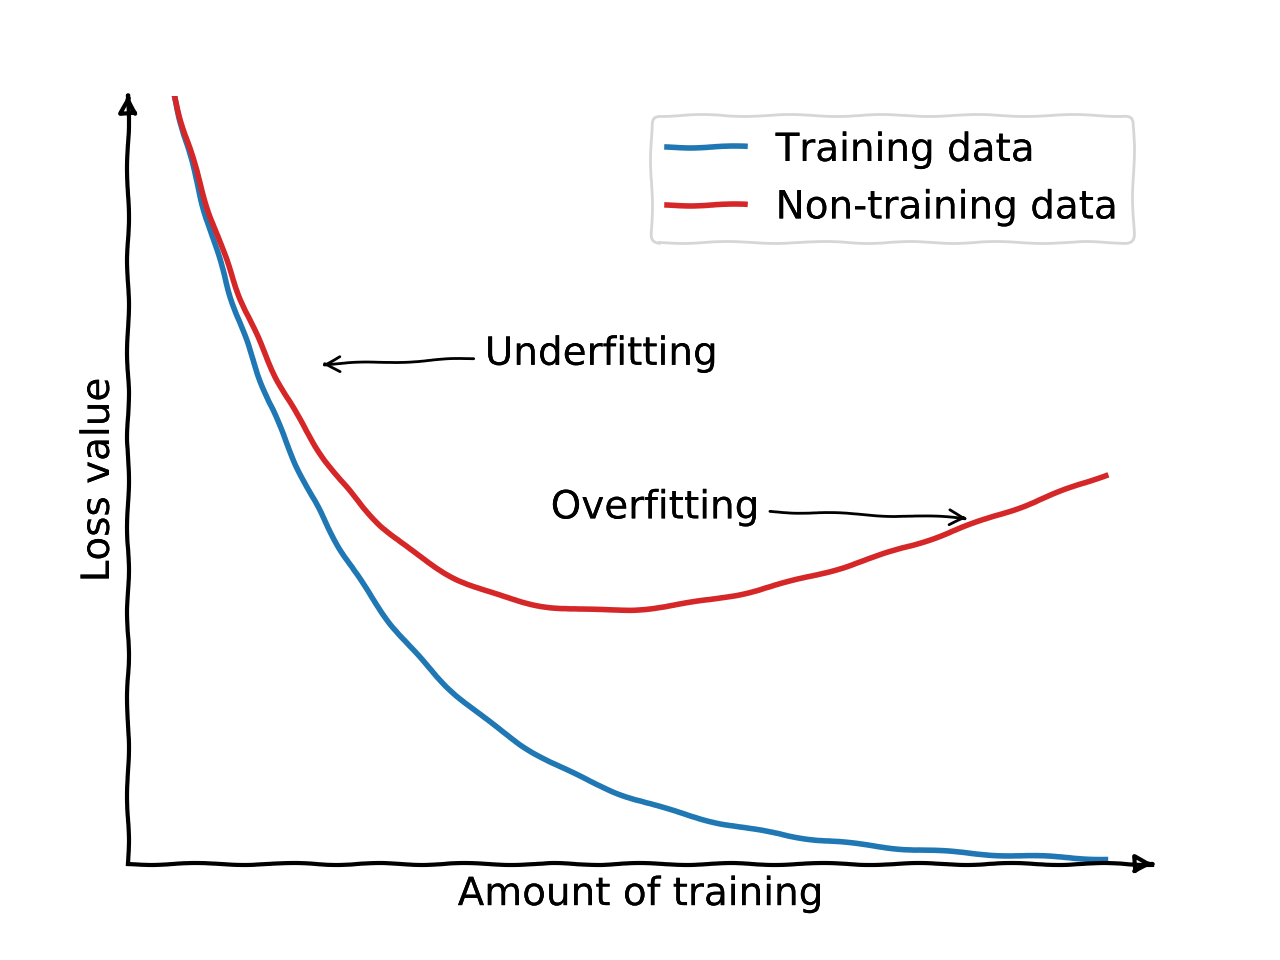
\includegraphics[width=\graphw, height=\graphh, keepaspectratio, trim = 1cm 5mm 1cm 1cm, clip]{\PhDthesisdir/plots_and_images/my_plots/ML/overfitting_and_early_stopping/overfitting_explained-5.png}
\end{center}
\end{frame}

\begin{frame}\addtocounter{framenumber}{-1}
\begin{center}
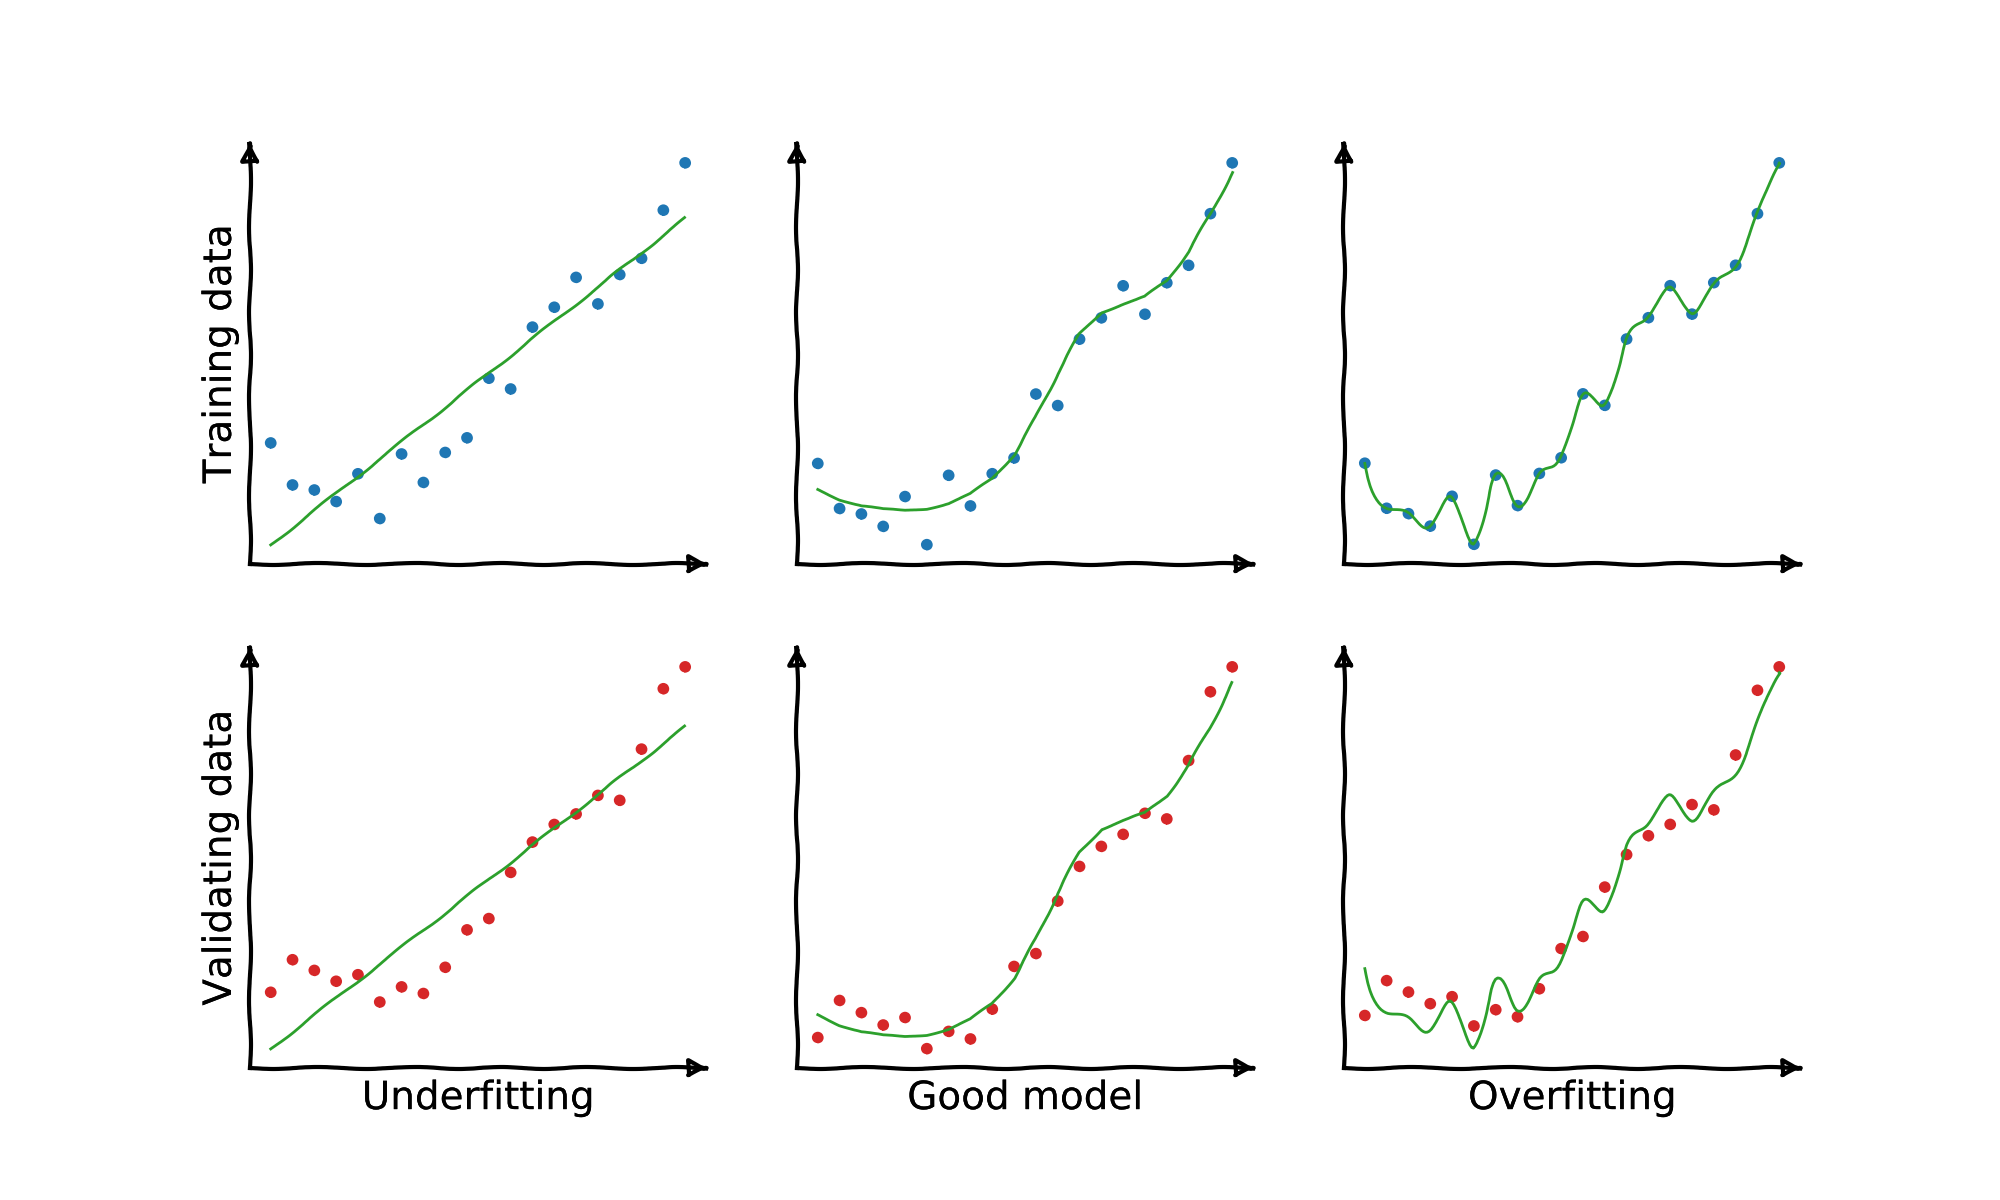
\includegraphics[width=\graphw, height=\graphh, keepaspectratio, trim = 1cm 1cm 1cm 1cm, clip]{\PhDthesisdir/plots_and_images/my_plots/ML/overfitting_and_early_stopping/examples_xkcd.png}
\end{center}
\end{frame}

\begin{frame}\addtocounter{framenumber}{-1}
\begin{center}
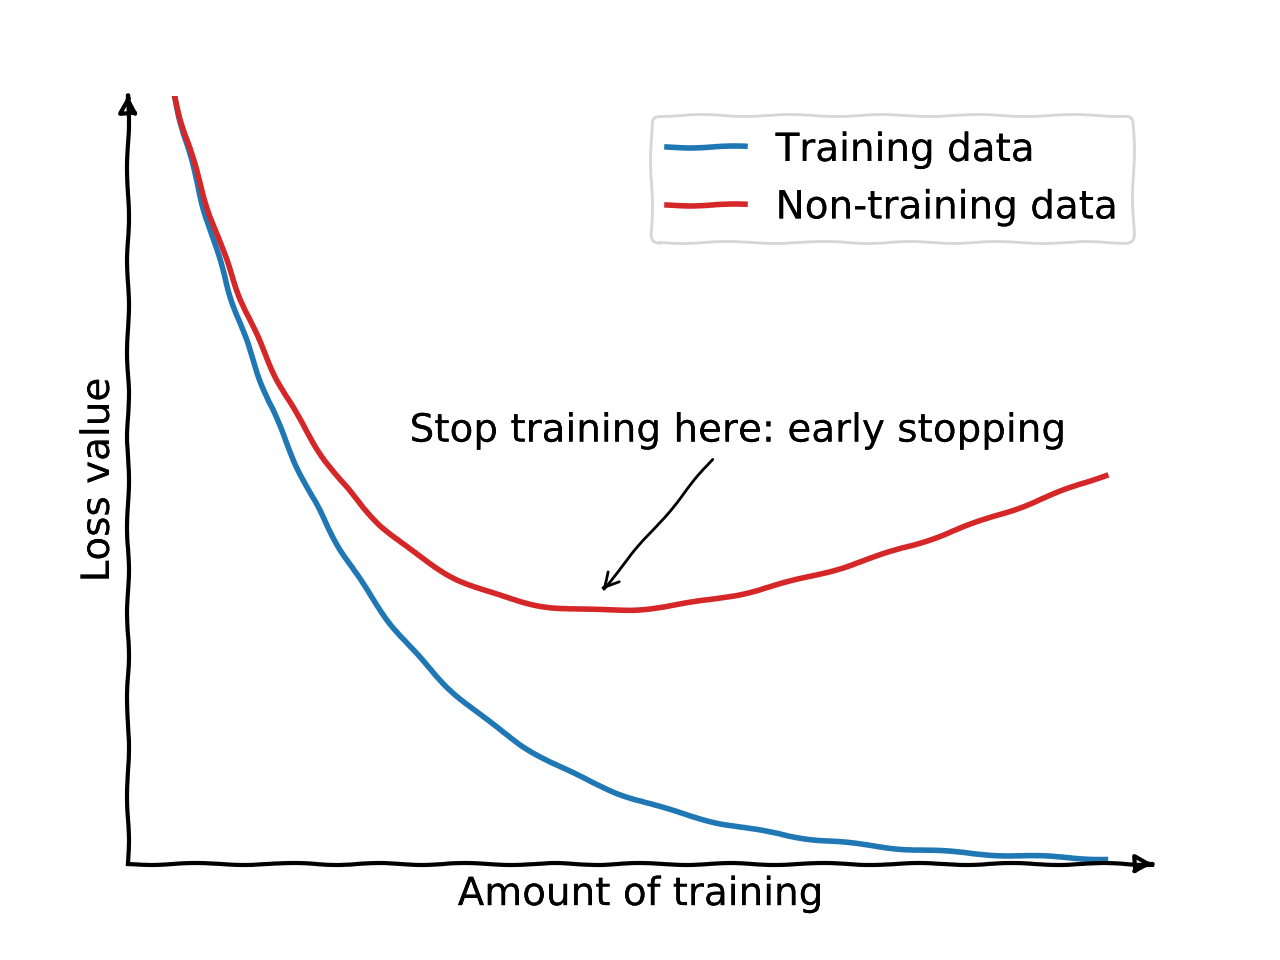
\includegraphics[width=\graphw, height=\graphh, keepaspectratio, trim = 1cm 5mm 1cm 1cm, clip]{\PhDthesisdir/plots_and_images/my_plots/ML/overfitting_and_early_stopping/overfitting_explained-6.png}
\end{center}
\end{frame}
\begin{frame}\addtocounter{framenumber}{-1}
\begin{center}
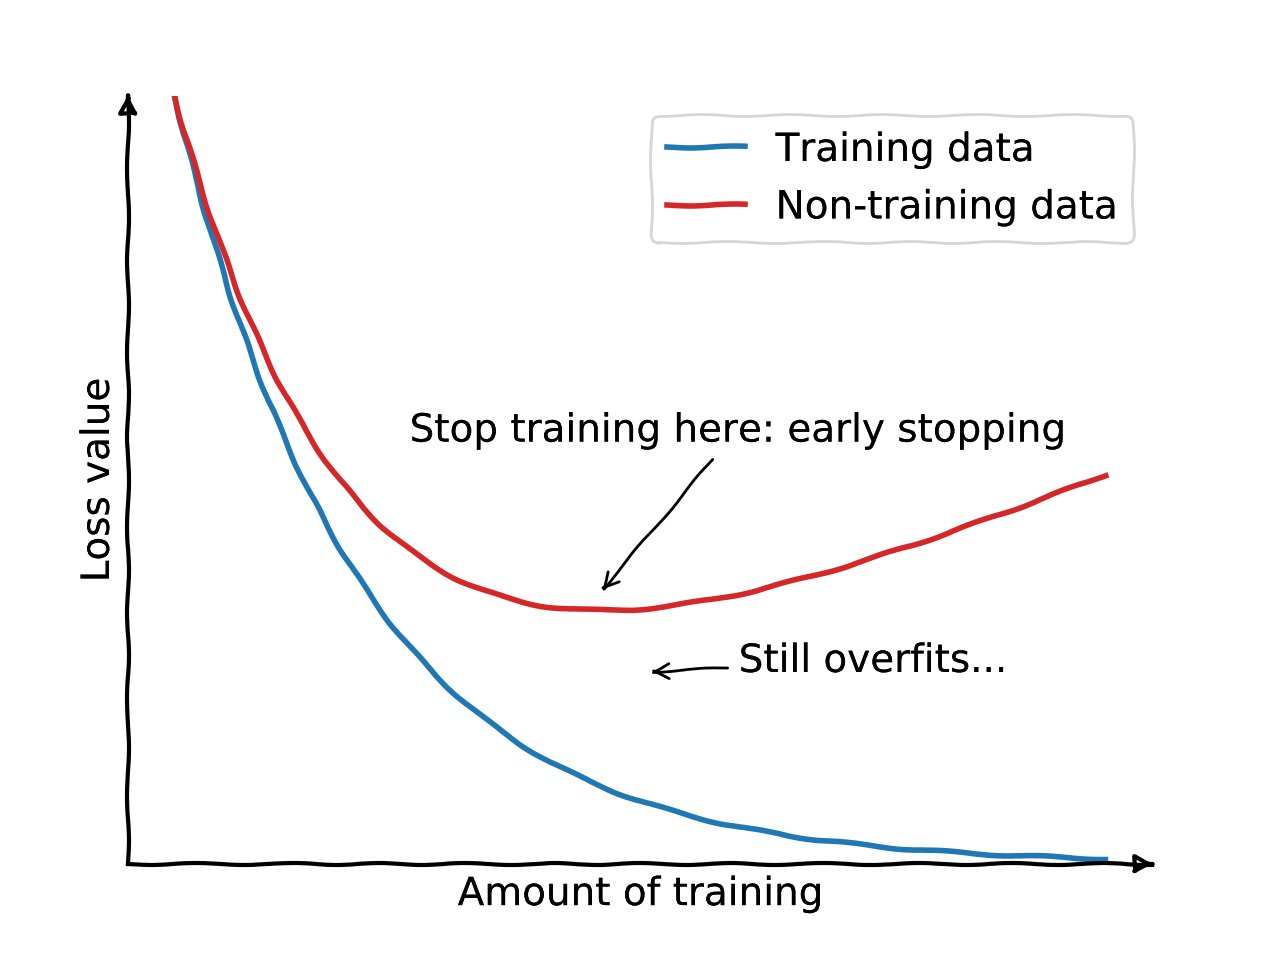
\includegraphics[width=\graphw, height=\graphh, keepaspectratio, trim = 1cm 5mm 1cm 1cm, clip]{\PhDthesisdir/plots_and_images/my_plots/ML/overfitting_and_early_stopping/overfitting_explained-7.png}
\end{center}
\end{frame}
\begin{frame}\addtocounter{framenumber}{-1}
\begin{center}
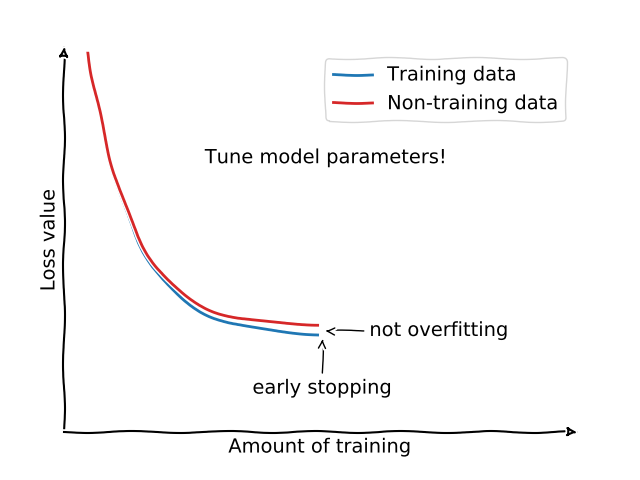
\includegraphics[width=\graphw, height=\graphh, keepaspectratio, trim = 1cm 5mm 1cm 1cm, clip]{\PhDthesisdir/plots_and_images/my_plots/ML/overfitting_and_early_stopping/overfitting_explained-8.png}
\end{center}
\end{frame}
